\documentclass[headrule,footrule]{foils}

%%
%%%  Macros
%%%
%%% fonts-sil-charis for IPA in week 5

\newcommand{\logo}{HG2002 (2021)}
\usepackage[hidelinks]{hyperref}

\newcommand{\header}[3]{%
  \title{\vspace*{-2ex} \large 
    HG2002 Semantics and Pragmatics
% \thanks{Creative
%       Commons Attribution License: 
%       you are free to share and adapt as long as you give 
%       appropriate credit and add no additional restrictions: 
%       \protect\url{https://creativecommons.org/licenses/by/4.0/}.
%     }
    \\[2ex] \Large  \emp{#2} \\ \emp{#3}}
  \author{\blu{Francis Bond}   \\ 
    \normalsize  \textbf{Division of Linguistics and Multilingual Studies}\\
    \normalsize  \url{http://www3.ntu.edu.sg/home/fcbond/}\\
    \normalsize  \texttt{bond@ieee.org}}
  \MyLogo{\logo}
  % \MyLogo{奈良女子大学:欧米言語情報理論II}
  \date{#1
    \\  \url{https://bond-lab.github.io/Semantics-and-Pragmatics/}
\\[.5ex] \footnotesize Creative  Commons Attribution License:  you are free to share and adapt 
\\[-.25ex] \footnotesize   as long as you give    appropriate credit and add no
additional restrictions: 
\\ \small  \protect\url{https://creativecommons.org/licenses/by/4.0/}.
}
  % \renewcommand{\logo}{#2}
  % \special{! /pdfmark where
  %   {pop} {userdict /pdfmark /cleartomark load put} ifelse
  %   [ /Author (Francis Bond)
  %   /Title (#1: #2)
  %   /Subject (HG2002: Semantics and Pragmatics)
  %   /Keywords (Semantics, Pragmatics, Meaning)
  %   /DOCINFO pdfmark}
  %   }
  \hypersetup{%
    final       = true,
    colorlinks  = true,
    urlcolor    = blue,
    citecolor   = blue,
    linkcolor   = MidnightBlue,
    unicode     = true,
    pdfauthor   = {Francis Bond},
    pdfkeywords = {Semantics, Pragmatics, Meaning},
    pdftitle    = {#1: #2},
    pdfsubject  = {HG2002 Semantics and Pragmatics; License CC BY 4.0}
  }
}


\usepackage[a4paper,landscape]{geometry}
%\usepackage[dvips]{xcolor}
\usepackage[dvipsnames,x11names]{xcolor}
\usepackage{graphicx}
\newcommand{\blu}[1]{\textcolor{blue}{#1}}
\newcommand{\grn}[1]{\textcolor{green}{#1}}
\newcommand{\hide}[1]{\textcolor{white}{#1}}
\newcommand{\emp}[1]{\textcolor{red}{#1}}
\newcommand{\txx}[1]{\textbf{\textcolor{blue}{#1}}}
\newcommand{\lex}[1]{\textbf{\mtcitestyle{#1}}}


\usepackage{amsmath,latexsym}
\usepackage{pifont}
\renewcommand{\labelitemi}{\textcolor{violet}{\ding{227}}}
\renewcommand{\labelitemii}{\textcolor{purple}{\ding{226}}}

\newcommand{\subhead}[1]{\noindent\textbf{#1}\\[5mm]}

\newcommand{\Bad}{\emp{\raisebox{0.15ex}{\ensuremath{\mathbf{\otimes}}}}}
\newcommand{\bad}{*}

\newcommand{\com}[1]{\hfill \textnormal{(\emp{#1})}}%
\newcommand{\cxm}[1]{\hfill \textnormal{(\txx{#1})}}%
\newcommand{\cmm}[1]{\hfill \textnormal{(#1)}}%

\usepackage{relsize,xspace}
\newcommand{\into}{\ensuremath{\rightarrow}\xspace}
\newcommand{\ent}{\ensuremath{\Rightarrow}\xspace}
\newcommand{\nent}{\ensuremath{\not\Rightarrow}\xspace}
\newcommand{\tot}{\ensuremath{\leftrightarrow}\xspace}
\usepackage{url}
\newcommand{\lurl}[1]{\MyLogo{\url{#1}}}

\usepackage{mygb4e}
\let\eachwordone=\itshape
\newcommand{\lx}[1]{\textbf{\textit{#1}}}
\newcommand{\ix}{\ex\it}

\newcommand{\cen}[2]{\multicolumn{#1}{c}{#2}}
%\usepackage{times}
%\usepackage{nttfoilhead}
\newcommand{\myslide}[1]{\foilhead[-25mm]{\raisebox{12mm}[0mm]{\emp{#1}}}\MyLogo{\logo}}
\newcommand{\myslider}[1]{\rotatefoilhead[-25mm]{\raisebox{12mm}[0mm]{\emp{#1}}}}
%\newcommand{\myslider}[1]{\rotatefoilhead{\raisebox{-8mm}{\emp{#1}}}}

\newcommand{\section}[1]{\myslide{}{\begin{center}\Huge \emp{#1}\end{center}}}



\usepackage[lyons,j,e,k]{mtg2e}
\renewcommand{\mtcitestyle}[1]{\textcolor{teal}{\textsl{#1}}}
%\renewcommand{\mtcitestyle}[1]{\textsl{#1}}
\newcommand{\ja}[1]{\mtcitestyle{\makexeCJKactive #1\makexeCJKinactive}}
\newcommand{\chn}{\mtciteform}
\newcommand{\zsm}{\mtciteform}
%\newcommand{\cmn}[1]{make\cjkactive\mtciteform#1\makecjkinactive}
\newcommand{\iz}[1]{\textup{\texttt{\textcolor{blue}{\textbf{#1}}}}}
\newcommand{\con}[1]{\textsc{#1}}
\newcommand{\gm}{\textsc}
\newcommand{\cmp}[1]{{[\textsc{#1}]}}
\newcommand{\sr}[1]{\ensuremath{\langle}#1\ensuremath{\rangle}}
\usepackage[normalem]{ulem}
\newcommand{\ul}{\uline}
\newcommand{\ull}{\uuline}
\newcommand{\wl}{\uwave}
\newcommand{\vs}{\ensuremath{\Leftrightarrow}~}
%%% theta role
\newcommand{\tr}[1]{\textcolor{Chartreuse4}{\textsc{#1}}}
%%% theta grid
\newcommand{\grid}[1]{\ensuremath{\langle}\tr{#1}{\ensuremath{\rangle}}}

%%%
%%% Bibliography
%%%
\usepackage{natbib}
%\usepackage{url}
\usepackage{bibentry}
%\usepackage{CJKutf8}


\usepackage{fontenc}
\usepackage{polyglossia}
\setmainlanguage{english}
\setotherlanguages{tamil}
\setmainfont[Ligatures=TeX]{TeX Gyre Pagella}
\setsansfont[Ligatures=TeX]{TeX Gyre Heros}
\newfontfamily\ipafont{Charis SIL}
\newcommand\ipa[1]{\mtcitestyle{\ipafont #1}}


\usepackage{xeCJK}
\makexeCJKinactive
\newcommand{\zh}[1]{\mtcitestyle{\makexeCJKactive #1\makexeCJKinactive}}
%\newcommand{\ja}[1]{\makexeCJKactive #1\makexeCJKinactive}
\setCJKmainfont{Noto Sans CJK JP}
\setCJKsansfont{Noto Sans CJK SC}
\setCJKmonofont{Noto Sans CJK SC}

\newfontfamily\tamilfont[Script=Tamil]{Noto Sans Tamil}
\newfontfamily\tamilfontsf[Script=Tamil]{Noto Sans Tamil}
\newcommand{\tam}[1]{\texttamil{#1}}
%%% From Tim
\newcommand{\WMngram}[1][]{$n$-gram#1\xspace}
\newcommand{\infers}{$\rightarrow$\xspace}


\usepackage{rtrees,qtree}
\renewcommand{\lf}[1]{\br{#1}{}}
\usepackage{avm}
%\avmoptions{topleft,center}
\newcommand{\ft}[1]{\textsc{#1}}
\renewcommand{\val}[1]{\textit{#1}}
\newcommand{\typ}[1]{\textit{#1}}
\avmfont{\sc}
\avmvalfont{\sc}
\renewcommand{\avmtreefont}{\sc}
\avmsortfont{\it}


%%% From CSLI book
\newcommand{\mc}{\multicolumn}
\newcommand{\HD}{\textbf{H}\xspace}
\newcommand{\el}{\< \>}
\makeatother
\long\def\smalltree#1{\leavevmode{\def\\{\cr\noalign{\vskip12pt}}%
\def\mc##1##2{\multispan{##1}{\hfil##2\hfil}}%
\tabskip=1em%
\hbox{\vtop{\halign{&\hfil##\hfil\cr
#1\crcr}}}}}
\makeatletter

%\usepackage{tipa}
\usepackage{multicol}


\newcommand{\task}{\marginpar{\large ~~~\textbf{?}}}
\newcommand{\sh}[1]{\href{https://www.arthur-conan-doyle.com/index.php?title=#1}{#1}}

\usepackage{tikz}
\usepackage{tikz-qtree}
\usepackage{forest}

% \usepackage{tree-dvips}
% \newcommand{\sa}[2]{\node{c#1}{\iz{#2}}}%\nodebox{c#1}}
% \usepackage{pst-node}
% \usepackage{pst-plot}

% \usepackage{tree-dvips} % ALT Ontology
% \newcommand{\sa}[2]{\rnode{c#1}{\iz{#2}}} %\nodebox{c#1}}
% %\newcommand{\sagt}[2]{\rnode{c#1}{\iz{#2}}} %\nodebox{c#1}}
% \newcommand{\sagt}[2]{\rnode{c#1}{\izn{#1}{#2}}} %\nodebox{c#1}}
% \newcommand{\izn}[2]{\iz{#1:#2}}



\begin{document}
%\begin{CJK}{UTF8}{min}
\header{Lecture 11}{Cognitive linguistics}{}\maketitle

%\include{schedule}

\myslide{Overview}
\begin{itemize}\addtolength{\itemsep}{-2ex}
\item Revision: Formal Semantics
\begin{itemize}
%  \item Logical Metalanguage
%  \item Semantics and Models
  \item Quantifiers and Higher Order Logic
  \item Dynamic Approaches to Discourse
  \end{itemize}
\item Metaphor
\item Metonymy
\item Image Schemas
\item Polysemy
\item Mental Spaces
%\item Langacker’s Cognitive Grammar
\item Next and Final Lecture: \emp{Wrap-up and Revision} 
\\ \textbf{No Tutorial Problems}
\end{itemize}

 
%%%
%%% this changes each year, so keep separate
%%%

%\input{schedule}
% \begin{center}
% Finish Annotation by 17:00 Oct 21st; Submit Report by 17:00 Nov 4  
% \end{center}

%\MyLogo{}



\section{Revision: Formal Semantics}

% \myslide{Language meets Logic (again)}

% \begin{itemize}
% \item \txx{formal semantics} is also known as
%   \begin{itemize}
%   \item \txx{truth-conditional semantics}
%   \item \txx{model-theoretic semantics}
%   \item \txx{Montague Grammar}
%   \item \txx{logical semantics}
%   \end{itemize}
% \item A general attempt to link the meaning of sentences to the
%   circumstances of the world: \txx{correspondence theory}
%   \begin{itemize}
%   \item If the meaning of the sentence and the state of the world
%     \emp{correspond} then the sentence is \textbf{true}
%   \end{itemize}
% \end{itemize}

% \myslide{Model-Theoretical Semantics}

% \begin{enumerate}
% \item Translate from a natural language into a logical language
%   with explicitly defined syntax and semantics
% \item Establish a mathematical model of the situations that the
%   language describes
% \item Establish procedures for checking the mapping between the
%   expressions in the logical language and the modeled situations.
% \end{enumerate}


% \myslide{Translating English into a Logical Metalanguage}
% %\myslide{Empirical truths and connectives}
% \MyLogo{Recall lecture 4}
% \begin{itemize}
% \item Consider simple sentences
%   \begin{itemize}
%   \item Represent the predicates by a capital \txx{predicate letter}
%     \\ these can be n-ary
%   \item Represent the \txx{individual constants} by lower case letters
%   \item Represent \txx{variables} by lower case letters (x,y,z)
%   \end{itemize}
% \item Join simple sentences with logical connectives
% \\ treat relative clauses as \txx{and}
%   \begin{exe}
%     \ex \eng{Bobbie who is asleep writhes}: A(b) $\wedge$ W(b)
%     \ex \eng{Bobbie is asleep and Freddie drinks}: A(b) $\wedge$ D(f)
%     \ex \eng{Freddie drinks and sleeps}: D(f) $\wedge$ S(f)
%     \ex \eng{Freddie doesn't drink beer}: $\neg$ D(f,b)
%     \ex \eng{If Freddie drinks whiskey Bobbie sleeps}: D(f,w) \into S(b)
% %    \ex \eng{x is asleep}: A(x)
%   \end{exe}
% \end{itemize}

% \myslide{Quantifiers in Predicate Logic}
% \MyLogo{$\forall$ and \into; $\exists$ and $\wedge$}

% \begin{itemize}
%   \item Quantifiers bind variables and scope over predications
%     \begin{itemize}
%     \item \txx{Universal Quantifier} ($\forall$: \eng{each, every, all})
%     \item \txx{Existential Quantifier} ($\exists$: \eng{some, a})
%     \end{itemize}
%     \begin{exe}
%       \ex \eng{All students learn logic}: $\forall$x (S(x)  $\into$ L(x,l))
%       \ex \eng{A student learns logic}: $\exists$x (S(x)  $\wedge$ L(x,l))
%       \ex \eng{Some students learn logic}: $\exists$x (S(x)  $\wedge$ L(x,l))
%       \ex \eng{No students learn logic}: $\neg\exists$x (S(x)  $\wedge$ L(x,l))
%       \ex \eng{All students don't learn logic}: $\forall$x (S(x)  $\into$ $\neg$L(x,l))
%     \end{exe}
%   \item All variables must be bound
% \end{itemize}

% \myslide{Some Advantages in Translating to Predicate Logic}
% \MyLogo{}

% \begin{itemize}
% \item Explicit representation of scope ambiguity
%   \begin{exe}
%     \ex \eng{Everyone doesn't love semantics}
%     \begin{xlist}
%           \ex \eng{It is not the case that all people love semantics}:  
%           \\ $\neg\forall$x (L(x,s))
%           \ex \eng{All people have the property of not loving semantics}: 
%           \\ $\forall$x($\neg$L(x,s))
%     \end{xlist}
%   \end{exe}
% \item But the big advantage is in reasoning with the real world
%    \\ \txx{denotational semantic analysis}
% \end{itemize}


% \myslide{Creating a \txx{Model}}

% \begin{enumerate}\addtolength{\itemsep}{-1.5ex}
% \item a \txx{semantic interpretation} of the symbols of the predicate logic
% \item a \txx{domain}: the model of a situation which identifies the
%   linguistically relevant entities, properties and relations
% \item a \txx{denotation assignment function}: this is a procedure
%   which matches the linguistic elements with the items  that they denote (a \txx{naming function})
% \end{enumerate}
% \begin{itemize}
% \item Is the denotation correct (does it match the real world)?
%   \begin{itemize}
%   \item \textbf{Sentence} 
%     $p$ is true in situation $v$ if it corresponds with the real world: 
%     \\ {[$p$]$^v$ = 1}: the denotatum of $p$ in $v$ is true
%   \item \textbf{Constant} denotation of a constant is the individual entity in question
%   \item \textbf{Predicate constants} are sets of individuals for which the predicate holds
% \\ {\{$<x, y, z>$: $x$ hands $y$ to $z$\}}
%   \end{itemize}

% \end{itemize}

% \myslide{The Domain}

% \begin{itemize}
% \item The domain represents the individuals and representations in a situation $v$
% \item Combine this with an assignment function $F$ to form a model
% \\ $M_1 = <U_1, F_1>$ (or set of models: $M_2 = <U_1, F_2>$, \ldots)
% \end{itemize}

% \myslide{Evaluating a simple statement}
% \begin{itemize}
% \item How can we check if \eng{Ian sings},   S(i), is true?
%   \begin{itemize}
%   \item {[S(i)]$^{M_1}$ = 1 iff [i]$^{M_1} \in$ [S]$^{M_1}$} \\ The
%     sentence is true if and only if the extension of \eng{Ian} is part of
%     the set defined by \eng{sings} in the model $M_1$
%   \item $F_1$(i) = Ian; $F_1$(S) =   \{Ian, Peter\};  Ian $\in$  \{Ian, Peter\}
%   \item[$\Rightarrow$] [S(i)]$^{M_1}$ = 1
%   \end{itemize}
% \item \eng{Did Martin produce everyone in Joy Division}
%   \begin{itemize}
%   \item $\forall$x (J(x) $\wedge$ O(m,x))
%     \begin{itemize}
%     \item i $\wedge$ O(m,i) = ?; b $\wedge$ O(m,b) = ?;  p $\wedge$ O(m,p) = ?;
%       s $\wedge$ O(m,s) = ?
%     \end{itemize}
%   \item 1,1,1,1  = ?
%   \item[$\Rightarrow$] [$\forall$x (J(x) $\wedge$ O(m,x))] = 1  \hfill Yes
%   \end{itemize}
% \end{itemize}


\myslide{Defining Relations using Logic}

\begin{itemize}
\item \txx{hyponymy}
  \begin{itemize}
  \item $\forall$x(DOG(x) \into\ ANIMAL(x))
  \end{itemize}
\item \txx{antonym}
  \begin{itemize}
  \item $\forall$x(DEAD(x) \into\ $\neg$ALIVE(x))
  \item $\forall$x(ALIVE(x) \into\ $\neg$DEAD(x))
  \end{itemize}
\item \txx{converse}
  \begin{itemize}
  \item $\forall$x$\forall$y(PARENT(x,y) \into\ CHILD(y,x))
  \end{itemize}
\item \txx{synonym}
  \begin{itemize}
  \item $\forall$x((EGGPLANT(x) \into\ BRINJAL(x)) $\wedge$ 
    (BRINJAL(x) \into EGGPLANT(x)))
  \end{itemize}
\end{itemize}



\myslide{Restricted Quantifiers}

\begin{itemize}
\item \eng{Most students read a book}
  \begin{itemize}
  \item Most(x)(S(x) $\wedge$ R(x))
    \\ \eng{most things are students and most things read books}
  \item Most(x)(S(x) iff R(x))
    \\ \eng{most things, if they are students, read books}
    \\ but also true for all things that are not students!
  \end{itemize}
\item We need to restrict the quantification
  \begin{itemize}
  \item (Most x: (S(x)) R(x)
  \end{itemize}
\item Sometimes we need to decompose
  \begin{itemize}
  \item \eng{everybody} ($\forall$x: (P(x))
  \item \eng{something} ($\exists$x: (T(x))
  \end{itemize}
\end{itemize}

% \myslide{Higher Order Logic}
%  \begin{itemize}
% \item Recall  \eng{Ian sings}
%   \begin{itemize}
%   \item {[S(i)]$^{M_1}$ = 1 iff [i]$^{M_1} \in$ [S]$^{M_1}$} \\ The
%     sentence is true if and only if the extension of \eng{Ian} is part of
%     the set defined by \eng{sings} in the model $M_1$
%   \item Remodel, with sing a property of Ian: i(S) \\ {[i(S)]$^{M_1}$
%       = 1 iff [S]$^{M_1} \in$ [i]$^{M_1}$} \\ The sentence is true if
%     and only if the denotation of the verb phrase \textit{sings} is
%     part of the extension of \eng{Ian}  in the model $M_1$
%   \end{itemize}
% \item \eng{Ian} is a set of sets of properties: \txx{second-order logic}
% \end{itemize}

\myslide{Generalized Quantifiers} 

\begin{itemize}
\item Q(A,B): \eng{Q A are B}
\item most(A,B) =1 iff $|$ A $\cap$ B $| > |$ A $-$ B $|$ 
\item all(A,B) =1 iff  A $\subseteq$ B  
\item some(A,B) =1 iff  A $\cap$ B $\ne \emptyset$ 
\item no(A,B) =1 iff A $\cap$ B  $= \emptyset$ 
\item fewer than x(A,B,X) =1 iff $|$ A $\cap$ B $| <  |$ X $|$ 
\end{itemize}

\myslide{Strong/Weak Quantifiers}

\begin{exe}
  \ex only \txx{weak} quantifiers can occur in existential \eng{there} sentences
  \begin{xlist}
    \ix There is a fox in the henhouse
    \ix There are two foxes in the henhouse
    \ix *There is every fox in the henhouse
    \ix *There are both foxes in the henhouse
  \end{xlist}
\end{exe}
\begin{itemize}
\item \txx{symmetrical} (cardinal) quantifiers are \txx{weak}
  \\ det(A,B) = det(B,A)
  \begin{exe}
    \ex \eng{three lecturers are Australian}   = \eng{three Australians are lecturers}
  \end{exe}
\end{itemize}

\myslide{Negative Polarity Items}

\begin{itemize}
\item Some words in English appear only in downward entailing expressions
  \begin{itemize}
  \item \txx{Upward entailment} goes from a subset to a set
  \item \txx{Downward entailment} goes from a set to a subset
  \end{itemize}
\end{itemize}
\begin{exe}
  \ex
  \begin{xlist}
    \ex \eng{Kim does\ull{n't} eat dessert} \ent  \eng{Kim does\ull{n't} eat hot dessert}
    \ex \eng{Kim does\ull{n't} eat hot dessert} \nent  \eng{Kim does\ull{n't} eat dessert}
    \trans \textbf{Downward entailment}
    \end{xlist}
    \ex
  \begin{xlist}
    \ex \eng{Kim eats some desserts} \nent  \eng{Kim eats hot dessert}
    \ex \eng{Kim eats some hot dessert} \ent  \eng{Kim  eats some desserts}
    \trans \textbf{Upward entailment}
    \end{xlist}
  \end{exe}
  \begin{itemize}
  \item Negative Polarity Items are licensed by downward entailing expressions
  \end{itemize}


\myslide{Left and Right Monotonicity}

\begin{itemize}
\item The monotonicity may depend on the position
  \begin{exe}
    \ex 
 \begin{xlist}
    \ex \eng{Every student studies semantics} \nent  
    \eng{Every student studies formal semantics}
    \ex \eng{Every student studies formal semantics} \ent  
    \eng{Every student studies semantics}
    \trans \textbf{Upward entailment (right argument)}
    \end{xlist}
    \ex 
 \begin{xlist}
    \ex \eng{Every student studies semantics} \ent  
    \eng{Every linguistics student studies  semantics}
    \ex \eng{Every linguistic student studies  semantics} \nent  
    \eng{Every student studies semantics}
    \trans \textbf{Downward entailment (left argument)}
    \end{xlist}
\newpage
  \ex 
 \begin{xlist}
    \ex \eng{Every student who has ever studied semantics loves it}
    \ex *\eng{Every student who has studied semantics ever loves it}
    \ex \eng{Few students who have ever studied semantics dislike it}
    \ex \eng{Few students who have studied semantics ever dislike it}
    \end{xlist}
  \end{exe}
\end{itemize}
\begin{itemize}
\item Formal models of quantification can be used to make predictions
  about seemingly unrelated phenomena
\end{itemize}

\myslide{Modality as a scale of Implicatures}
\MyLogo{Allan (1986): incomplete}

\begin{exe}
  \ex \eng{I know that $p$}
  \ex \eng{I am absolutely certain that  $p$}
  \ex \eng{I am almost certain that  $p$}
  \ex \eng{I believe that $p$}
  \ex \eng{I am pretty certain that $p$}
\\ $\ldots$
\item \eng{Possibly $p$}
\\ $\ldots$
  \ex \eng{It is very unlikely that $p$}
  \ex \eng{It is almost impossible that  $p$}
  \ex \eng{It is impossible that $p$}
  \ex \eng{It is not the case that $p$}
  \ex \eng{I am absolutely certain that  not-$p$}
\end{exe}

\myslide{Modal Logics}

\begin{itemize}
\item Add modal operators
  \begin{itemize}
  \item Epistemic
    \begin{itemize}
    \item $\operatorname\Diamond\phi =$ \eng{it is possible that $\phi$}
    \item $\operatorname\Box\phi =$ \eng{it is necessary that $\phi$}
    \end{itemize}
  \item Deontic
    \begin{itemize}
    \item $\operatorname{P}\phi =$ \eng{it is permitted that $\phi$}
    \item $\operatorname{O}\phi =$ \eng{it is obligatorily $\phi$}
    \end{itemize}
  \end{itemize}
\item Define them in terms of \txx{possible worlds}
  \begin{itemize}
  \item $\operatorname{\Diamond}\phi$: true in at least one world
  \item $\operatorname{\Box}\phi$: true in all worlds
  \item $\operatorname{P}\phi$: true in at least one legal or morally ideal world
  \item $\operatorname{O}\phi$: true in all legal or morally ideal worlds
  \end{itemize}
\end{itemize}

\section{Cognitive Semantics}

\myslide{Introduction}

\begin{itemize}
\item Cognitive linguistics sees language as embedded in its use
  \begin{itemize}
  \item a \txx{functional} approach to language
  \item considering \txx{diachronic} and not just \txx{synchronic} evidence
  \item little or no separation between syntax, semantics and pragmatics
  \end{itemize}
\item The basic idea is that one thing is characterized in terms of another
  \begin{itemize}
  \item \txx{Metaphor} and \txx{figurative} language
  \item \txx{Image Schemas}
  \item \txx{Mental Spaces}
  \end{itemize}
\end{itemize}


\myslide{Figurative language use}

\begin{exe}
\ex \eng{Our new boss is a dinosaur}
\ex \eng{She fought for her life [in hospital]}
\ex \eng{His mind was racing}
\ex \eng{The ham skated across the kitchen floor}
\ex \eng{The brandy tobogganed down his throat}
\end{exe}
% \myslide{Metaphors}

% Natural culinary selection has led to the evolution of wildly
% varied pasta shapes – some estimates put it at well over 300- many
% of which were specifically designed to go with a particular kind of
% sauce.
% Generally, the more convoluted the pasta shape, the more
% sauce will cling to it, and the chunkier the sauce it can accompany.
% Strand pastas, such as spaghetti, are good all-rounders. Their
% slim strands are easily coated by thinner sauces, but when stirred
% and tangled together, they can also carry the thicker sauce.
% Ribbon pasta like fettuccine and linguine are even better at
% holding on to thicker sauces, especially if they have ruffled edges.
% Shaped pastas, like bowties, shells and wheels, typically have
% crevices, nooks and ridges that are great for catching chunky
% sauces. The larger types, such as conchiglioni, are big enough to fill
% with stuffing.
% Tube pastas run a very wide gamut of lengths, widths,
% twistiness and ruggedness, from everyone’s favourite , maccheroni,
% to long hollow buccatini, to fat ridged stuffable rigatoni
% Artisanal pasta (labelled artiginale) is more expensive than
% ordinary pasta, but worth it. It’s made in small batches from finest
% quality wheat, using bronze moulds which leave tiny microscopic
% ridges on the pasta surface that increase its ability to hold on to
% sauce.

\section{Metaphors}
\myslide{Metaphors and Mechanisms of Interpretation}

A metaphor is an extension of the use of a word beyond its
primary meaning to describe referents that bear similarities to
the word's primary referent.
\begin{itemize}
\item \lex{eye} ``body part used for vision''
  \begin{exe}
  \ex \eng{dull end of a needle (with a hole for the thread)} 
  \raisebox{-2.5ex}{
\includegraphics[width=3em]{pics/needle}}    
  \ex \eng{the bud on a potato}
\raisebox{-2ex}{
\includegraphics[width=3em]{pics/potato}}     
  \ex \eng{the centre of a storm} \raisebox{-4ex}{
\includegraphics[width=10em]{pics/eye-of-storm}}
  \end{exe}
\item The similarities between these referents and the primary referent of
the word \lex{eye} are their roundish shape and their more or less central
location on a larger shape.
\end{itemize}

% \myslide{Metaphors and Mechanisms of Interpretation}

% A metaphor is an extension of the use of a word beyond its
% primary meaning to describe referents that bear similarities to
% the word’s primary referent.
% \begin{itemize}
% \item \lex{eye} ``bo dy part used for vision'' 
%   \begin{exe}
%   \ex \eng{dull end of a needle (with a hole for the thread)}
%   \ex \eng{the bud on a potato}
%   \ex \eng{the centre of a storm}
%   \end{exe}
% \item The similarities between these referents and the primary referent of
% the word \lex{eye} are:
% \begin{itemize}
% \item roundish shape
% \item more or less central location on a larger shape
% \end{itemize}
% \end{itemize}

\myslide{Grammaticalization}
\begin{itemize}
\item Once a metaphor becomes accepted, speakers tend to view the
metaphorical meaning as separated from its primary meaning

\begin{exe}
  \ex \eng{booking a flight}
  \ex \eng{tabling a motion}
  \ex \eng{seeing the point}
  \ex \eng{stealing the headlines}
  \ex \eng{buying time}
\end{exe}
\item These are \txx{dead} or \txx{frozen metaphors}: we don't need to
  specially process them
\item We would expect to find them in a lexicon like wordnet
\end{itemize}

\myslide{Metaphors as non-prototypical use}

\begin{itemize}
\item In a way, metaphors are non-prototypical uses of a word.
\begin{itemize}
\item Humans understand words by referring to a prototypical usage,
and they match a new example against the characteristics of the
prototype.
\item  Use of words with broken typicality conditions happens all the
time.
\end{itemize}
\item
  \begin{exe}
    \ex \eng{The price of brussel sprouts went up.}
    \ex \eng{Marigold is coming out of a coma.}
    \ex \eng{Felix is under age.}
    \ex \eng{I killed his argument.}
    \ex \eng{Their love affair is blossoming.}
    \ex \eng{She has a fertile imagination.}
  \end{exe}
\item Depending on how you count frozen metaphors, 
we use metaphors more than literal uses
\end{itemize}

\myslide{Metaphors as central to understanding}
% \begin{exe}
%   \ex \eng{Her heart drummed against her rib-cage \ex \eng{The music flowed over
%   her \ex \eng{The evening staggered/plodded on
% \end{exe}

\begin{quote}
  \Large Our conceptual system is fundamentally
metaphorical in nature
\end{quote}
\begin{flushright}
  George Lakoff
\end{flushright}

\begin{itemize}
\item Cognitive semantics:
\\ There is no separation between cognition and
linguistic knowledge
\item Features of Metaphor
\begin{itemize}
\item \txx{Conventional} some metaphors are very well established (but
  remain metaphorical)
\item \txx{Systematic} understood as part of larger domains
\item \txx{Asymmetrical} normally understand the \emp{abstract} 
  in terms of the \emp{concrete} (and not the other way round)
\end{itemize}

\end{itemize}


\myslide{Metaphors we live by}

\begin{itemize}
\item Metaphor is pervasive in everyday life, not just in
language but in thought and action.
\item Our ordinary conceptual system, in terms of which we
both think and act, is fundamentally metaphorical in
nature.
\item If we are right in suggesting that our conceptual system
is largely metaphorical, then the way we think, what we
experience, and what we do every day is very much a
matter of metaphor.
\end{itemize}

\begin{quote}
  George Lakoff and Mark Johnson \citeyear{Lakoff:Johnson:1980} \textit{Metaphors we live by} 
  University of Chicago Press.
\end{quote}



\myslide{Prototypical metaphors}

Some metaphors are not as good as others because not all broken typicality
conditions result in prototypical metaphors. What is a prototypical
metaphor?

\begin{itemize}
\item Similarity and dissimilarity have both been stressed.
\item Items must not be too similar:
  \begin{exe}
    \ex \eng{$^\#$Wine is whisky}
    \ex \eng{$^\#$Cars are trucks}
    \ex \eng{$^\#$Jam is honey}
  \end{exe}
\newpage
\item They should not be too dissimilar:
  \begin{exe}
    \ex \eng{His feet were stars}
    \ex \eng{Her cheeks were typewriters}
    \ex \eng{Her knees were penguins}
  \end{exe}
\item In a prototypical metaphor then, items compared are
likely to come from different lexical fields but they are
also similar in that they do share some minor
characteristic. Dissimilarity signals the listener to do
some active semantic matching.
\begin{exe}
  \ex \eng{Life is a subway train}
  \ex \eng{Men are thistles}
  \ex \eng{He posted the toast down to his stomach}
\end{exe}
\end{itemize}

\myslide{Target and Source Domains}

% \begin{exe}
%   \ex \eng{The cake was absolutely wicked.
% \iz The chocolate crème was just plain sinful. I feel guilty eating it.
% \end{exe}
\begin{quote}
 Metaphors enable us to understand one
  domain of experience in terms of another.
\\ \mbox{}\hfill \citet{Lakoff:Turner:1989}
\end{quote}

\begin{itemize}
\item We map from a \txx{source domain} to a \txx{target domain}
\\[1.5ex] often written: \txx{TARGET} is \txx{SOURCE}
\end{itemize}




% \myslide{DESIRE is HUNGER}

% \begin{exe}
%   \ex \eng{She was drooling over him.}  
%   \ex \eng{He is sex-starved.}
%   \ex \eng{She thirsts for recognition.} 
%   \ex \eng{Her sexual appetite is enormous.}
%   \ex \eng{He hungers for her touch.}
% \end{exe}
% \begin{itemize}
% \item Target domain: SEX (DESIRE, LUST)
% \item Source domain: FOOD (HUNGER, EATING)
% \end{itemize}


\myslide{ARGUMENT is WAR}

\begin{exe}
\ex \eng{Your claims are indefensible.}
\ex \eng{He attacked every weak point in my argument.}
\ex \eng{His criticisms were right on target.}
\ex \eng{I demolished his argument.}
\ex \eng{I’ve never won an argument with him.}
\ex \eng{You disagree? Okay shoot!}
\ex \eng{If you use that strategy, he’ll wipe you out.}
\ex \eng{He shot down all my arguments.}
\ex \eng{He was defeated by the argument.}
\end{exe}
\newpage
\begin{itemize}
\item We don’t just talk about argument in terms of war. We can actually win or
lose arguments.
\item  Many of the things we do in arguing are partially structured by the concept of war.
Though there is no physical battle, there is a verbal battle.
\begin{itemize}
  \item  We see the person we are arguing with as an opponent.
  \item  We attack their positions and defend our own.
  \item  We gain and lose ground.
  \item  We plan and use strategies.
 \end{itemize}

\item The metaphor is not only in the words we use --- it is in our very concept of argument.  We talk about arguments that way because we conceive of them that way --- and we
act according to the way we conceive of things
\item But we could think of an argument as a search for truth, \ldots
\end{itemize}

\myslide{Argument: When losing is winning}
\MyLogo{\url{http://www.humansinvent.com/\#!/13260/argument-when-losing-is-winning/}}

\begin{itemize}
\item Leo Kent (2013) argues that the argument as war metaphor is counterproductive
  \begin{itemize}
  \item Suppose you and I have an argument. You believe a proposition, P, and I don’t. I’ve objected, I’ve questioned, I’ve raised all sorts of counter-considerations, and in every case you’ve responded to my satisfaction. At the end of the day, I say, ‘You know what? I guess you’re right.’
  \item So I have a new belief. And it’s not just any belief, but it’s a well-articulated, examined and battle-tested belief.
  \item So who won that argument? Well, the war metaphor seems to force us into saying you won, even though I’m the only one who made any cognitive gain.
  \item The war metaphor forces us into thinking that you’re the winner and I lost, even though I gained and there’s something wrong with that picture.
  \end{itemize}
  
\end{itemize}



\myslide{Spatial Metaphors}
\MyLogo{\textit{Backs to the Future} \url{http://ucsdnews.ucsd.edu/archive/newsrel/soc/backsfuture06.asp}}
\begin{itemize}
\item \txx{Spatial metaphors} have to do with
spatial orientation: \lex{up-down, in-out, front-back, on-off, deep-shallow, 
central-peripheral}.

\item Spatial metaphors give a concept a spatial orientation eg.
HAPPY is UP: \eng{I'm feeling up today}
\item Though polar oppositions \eng{up-down, in-out} are physical in nature, the spatial
metaphors based on them can vary from culture to culture. (e.g. in most 
cultures FUTURE is FRONT but in at least one FUTURE is BACK)
\begin{itemize}
\item Aymara, who live in the Andes highlands of Bolivia, Peru and
  Chile, have future behind them
\end{itemize}
\end{itemize}

\myslide{HAPPY is UP}
\begin{exe}
\ex \eng{I'm feeling up.}
\ex \eng{That boosted my spirits.}
\ex \eng{My spirits rose.}
\ex \eng{You're in high spirits.}
\ex \eng{Thinking about logic gives me a lift.}
\ex \eng{I'm feeling down.}
\ex \eng{I'm depressed.}
\ex \eng{He is really low these days.}
\ex \eng{I fell into a depression.}
\ex \eng{My spirits sank.}
\end{exe}



\myslide{HEALTHY is UP}
\begin{exe}
\ex \eng{He's at the peak of health.}
\ex \eng{Lazarus rose from the dead.}
\ex \eng{He's in top shape.}
\ex \eng{She fell ill.}
\ex \eng{He is sinking fast.}
\ex \eng{She came down with the flu.}
\ex \eng{Her health is declining.}
\ex \eng{He dropped dead.}
\end{exe}

\myslide{CONTROL is UP}
\begin{exe}
\ex \eng{I have control over them.}
\ex \eng{I am on top of the situation.}
\ex \eng{He's at the height of this power.}
\ex \eng{She's in high command.}
\ex \eng{He's in the upper echelon.}
\ex \eng{Her power rose.}
\ex \eng{He ranks above me in strength.}
\ex \eng{She is under my control.}
\ex \eng{He fell from power.}
\ex \eng{Her power is on the decline.}
\end{exe}

\myslide{AWAKE is UP}
\begin{exe}
\ex \eng{Get up.}
\ex \eng{Wake up.}
\ex \eng{I'm up already.}
\ex \eng{He rises early in the morning.}
\ex \eng{She fell asleep.}
\ex \eng{He dropped off to sleep.}
\ex \eng{Sje's under hypnosis.}
\ex \eng{He sank into a coma.}
\end{exe}

\myslide{VIRTUE is UP}
\begin{exe}
\ex \eng{He is high-minded.}
\ex \eng{She is upright.}
\ex \eng{She is a upstanding citizen.}
\ex \eng{He is underhanded.}
\ex \eng{I wouldn't stoop to that.}
\ex \eng{That is beneath me.}
\ex \eng{That was a low trick.}
\end{exe}

\myslide{MORE is UP}
\begin{exe}
\ex \eng{The number of books printed keeps going up.}
\ex \eng{The number of errors he made is incredibly low.}
\ex \eng{What is the upper bound?}
\end{exe}

\begin{itemize}
\item Our experience of physical objects and substances provides a
  further basis for understanding.
\item UP is positive
  \begin{itemize}
  \item if we pile things up, more reach higher
  \item healthy people stand upright
  \item when we are awake, we stand up
  \end{itemize}
\item Understanding our experiences
  in terms of objects and  substances allows us to pick out parts
  of our experience and treat them as discrete entities.
\end{itemize}

\myslide{MENTAL HEALTH is a (FRAGILE) OBJECT}
\begin{exe}
\ex \eng{Her mental health is very fragile.}
\ex \eng{We have to handle him with care since his wife's death.}
\ex \eng{He broke under cross-examination.}
\ex \eng{She is easily crushed.}
\ex \eng{The experience shattered him.}
\ex \eng{I'm going to pieces.}
\ex \eng{His mind snapped.}
\ex \eng{He cracked up.}
\end{exe}

\myslide{MIND is a MACHINE}
\begin{exe}
\ex \eng{We're still trying to grind out the solution to this equation.}
\ex \eng{My mind just isn't operating today.}
\ex \eng{Boy, the wheels are turning now!}
\ex \eng{I'm a little rusty today.}
\ex \eng{We've been working on this problem all day and now we're running out of  steam.}
\ex \eng{He broke down.}
\end{exe}

% \myslide{LOVE is FORCE}
% \begin{exe} 
% \ex \eng{I could feel the electricity between us,
% \ex \eng{There were sparks.
% \ex \eng{I was magnetically drawn to her.
% \ex \eng{They gravitate to each other.
% \ex \eng{The atmosphere around them is always charged etc.
% \end{exe}

% \myslide{LOVE is HEALTH}
% \begin{exe}
% \ex \eng{They have a strong healthy relationship.
% \ex \eng{Their love can't be revived.
% \ex \eng{Their love is on the mend etc.
% \end{exe}

% \myslide{LOVE is MADNESS}
% \begin{exe}
% \ex \eng{I'm crazy about him.
% \ex \eng{He drives me out of my mind.
% \ex \eng{He raves on about her.
% \ex \eng{I'm madly in love with her.
% \ex \eng{She is wild about Anne etc.
% \end{exe}
 
% \myslide{LOVE is MAGIC}
% \begin{exe} 
% \ex \eng{She cast her spell over me.
% \ex \eng{The magic is gone.
% \ex \eng{I was spellbound.
% \ex \eng{He had me in a trance.
% \ex \eng{I was entranced by him.
% \ex \eng{I'm charmed by here.
% \ex \eng{He is bewitching
% \end{exe}

% \myslide{LOVE is WAR}
% \begin{exe} 
% \ex \eng{James is known for his many conquests.
% \ex \eng{She fought for him, but but his mistress won out.
% \ex \eng{She fled from Jeff's advances.
% \ex \eng{He pursued her relentlessly.
% \ex \eng{She won his hand in marriage.
% \ex \eng{He is besieged by suitors.
% \ex \eng{He has to fend them off. 
% \end{exe}


\myslide{LIFE is a JOURNEY}
\begin{itemize}
\item The person leading a life is a traveler
\item Their purposes are destinations
\item The means for achieving purposes are routes
\item Difficulties in life are impediments to travel
\item Counsellors are guides
\item Progress is the distance traveled
\item Things you gauge your progress by are landmarks
\item Material resources and talents are provisions.
\end{itemize}

\myslide{ANGER}

\begin{itemize}\addtolength{\itemsep}{-1ex}
\item Emotions are often considered to be feelings alone, and
as such they are viewed as being devoid of conceptual
content.
\item In fact emotions have a fairly complex conceptual
structure which can be studied through metaphors.
\item Lakoff and Johnson's cultural model of anger
\\ Physiological effects of anger:
  \begin{itemize}
  \item Increased body heat
  \item Increased internal pressure
  \item Agitation
  \item Interference with accurate perception
  \item As anger increases, the physiological effect increases
  \item There is a limit beyond which the physiological effects of anger impair normal functioning.
\end{itemize}
\end{itemize}
\newpage
\begin{itemize}
\item Body heat:
  \begin{exe}
    \ex \eng{Don't get hot under the collar.}
    \ex \eng{Billy's a hothead.}
    \ex \eng{They were having a heated argument.}
    \ex \eng{She got all hot and bothered.}
  \end{exe}
  \item Internal pressure:
  \begin{exe}
    \ex \eng{When I found out, I almost burst a blood vessel.}
    \ex \eng{He almost had a hemorrhage.}
    \ex \eng{I exploded at them.}
  \end{exe}
\newpage
\item Redness in the face and neck area:
  \begin{exe}
    \ex \eng{She was scarlet with rage.}
    \ex \eng{He got red with anger.}
    \ex \eng{He was flushed with anger.}
  \end{exe}
\item Agitation
\begin{exe}
  \ex \eng{She was shaking with anger.}
  \ex \eng{I was hopping mad.}
  \ex \eng{He was quivering with rage.}
  \ex \eng{He's all worked up.}
 \ex \eng{She's all wrought up.}
\end{exe}
\newpage
\item Interference with accurate perception
\begin{exe}
  \ex \eng{She was blind with rage.}
  \ex \eng{I was beginning to see red.}
  \ex \eng{I was so mad I couldn't see straight.}
\end{exe}
\end{itemize}

\myslide{ANGER is HEAT}

\begin{itemize}
\item ANGER is HEAT forms the basis of the most
  general metaphors for anger
\item There are two versions to this metaphor,
  one where the heat is applied to fluid and
  the other where the heat is applied to
  solids.
\item The fluid version is more elaborated
\end{itemize}

\begin{itemize}
\item The body is a container for the emotions
\begin{exe}
  \ex \eng{He was filled with anger.}
  \ex \eng{She couldn't contain her joy.}
  \ex \eng{She was brimming with rage.}
  \ex \eng{Try to get the anger out of your system.}
\end{exe}
\item
The ANGER is HEAT metaphor when applied to fluids combines with the
metaphor the body is a container for the emotions to yield the central
metaphor of the system:
\item ANGER is HEAT OF A FLUID in a container.
\begin{exe}
  \ex \eng{You make my blood boil.}
  \ex \eng{Simmer down!}
  \ex \eng{I had reached the boiling point.}
  \ex \eng{Let him stew.}
  \ex \eng{She was seething with rage.}
\end{exe}

\item Similarly \lex{pissed off} is used only to refer to anger --- ``hot liquid under
pressure''
\item Cool and calm corresponds to the lack of anger.
\begin{exe}
  \ex \eng{Keep cool.}
  \ex \eng{Stay calm.}
\end{exe}

\item When The Intensity Of Anger Increases The Fluid Rises
\begin{exe}
  \ex \eng{His pent-up anger welled up inside him.}
  \ex \eng{She could feel her gorge rising.}
  \ex \eng{We got a rise out of him.}
  \ex \eng{My anger kept building up inside me.}
  \ex \eng{Pretty soon I was in a towering rage.}
\end{exe}
\newpage
\item We also know that intense heat produces steam and creates pressure on the
container. This yields the metaphorical entailments:
\item Intense Anger Produces Pressure On The Container
  \begin{exe}
    \ex \eng{He was bursting with anger.}
    \ex \eng{I could barely contain my rage.}
    \ex \eng{I could barely keep it in any more.}
    \ex \eng{He suppressed his anger.}
    \ex \eng{They turned their anger inward.}
    \ex \eng{He managed to keep his anger bottled up inside him.}
%    \ex \eng{He was blue in the face.}
\end{exe}
\newpage
\item  When the pressure on the container becomes too high, the container explodes.
\item When Anger Becomes Too Intense The Person Explodes
  \begin{exe}
    \ex \eng{When I told him, he just exploded.}
  \ex \eng{She blew up at me.}
  \ex \eng{We don't like your outbursts.}
  \ex \eng{She blew a fuse.}
  \ex \eng{He blew a gasket.}
  \ex \eng{He erupted.}
\end{exe}
\newpage
\item When A Person Explodes, Parts Of Them Go Up In The Air.
  \begin{exe}
  \ex \eng{I blew my stack.}
  \ex \eng{I blew my top.}
  \ex \eng{She flipped her lid.}
  \ex \eng{He hit the ceiling.}
  \ex \eng{I went through the roof.}
\end{exe}

\newpage

\item The central metaphor of Anger as heated fluid in a container indicate
that the anger scale is not open-ended, it has a limit. Just as hot
fluid in a closed container can only take so much heat before it
explodes, so we conceptualise the anger scale as having a limit
point. We can only bear so much anger before we explode.
\item The conceptual metaphors are motivated by our physiology
\item There may be cross-cultural differences
\item And there are many possible metaphors

\begin{itemize}
\item ANGER is FIRE
\item ANGER is INSANITY
\item ANGER is an OPPONENT
\item ANGER is a DANGEROUS ANIMAL
\end{itemize}

\end{itemize}


\myslide{Anger in Lamaholot}

ANGER is HOT SPICE
\begin{exe}
  \ex \gll one=k helo n-o'oN sili lia' \\
heart=1SG.POSS like 3SG.exist chilli ginger \\
\trans ``I am furious (lit. there exist chilli and ginger in my heart).''
\end{exe}

Adonara-Lamaholot is a small language spoken on Eastern part of Flores
Island, Solor Island, and Lembata Island of Eastern Indonesia.   From
the PhD thesis of Elvis Albertus bin Toni (NTU 2018).  




\myslide{Influence of Metaphors}
\begin{itemize}
% \item Polysemy FIXME
\item Verbs of perception
\\  \begin{tabular}{lcl}
    seeing & \into & understanding \\
    hearing & \into & obeying \\
    tasting & \into & choosing \\
    feeling & \into & emoting \\
    smelling & \into & disliking \\
  \end{tabular}
\item Literal meanings extend into metaphorical meanings
\item These become conventionalized
\item And then we have polysemy
\end{itemize}

\myslide{Metonymy as Metaphor}  %% FIXME add examples

\begin{itemize}
\item PART for WHOLE (synecdoche)
  \begin{exe}
    \ex \eng{Can you lend a hand?}
  \end{exe}
\item WHOLE for PART (synecdoche)
  \begin{exe}
    \ex \eng{NTU won the soccer.}
  \end{exe}
\item CONTAINER for CONTENT
  \begin{exe}
    \ex \eng{The lunch menu had five dishes.}
  \end{exe}
\item MATERIAL for OBJECT
  \begin{exe}
    \ex \eng{I won gold.}
   \end{exe}
\newpage
 \item PRODUCER for PRODUCT
  \begin{exe}
    \ex \eng{I'll get an IBM}
  \end{exe}
\item PLACE for INSTITUTION (toponym)
  \begin{exe}
    \ex \eng{Downing Street has made no comment}
  \end{exe}
 \item INSTITUTION for PEOPLE RESPONSIBLE
   \begin{exe}
     \ex \eng{Fairprice raised its prices.}
   \end{exe}
\item PLACE for EVENT
  \begin{exe}
    \ex \eng{Hiroshima changed our view of war.}
  \end{exe}
  \newpage
 \item CONTROLLER for CONTROLLED
   \begin{exe}
     \ex \eng{A truck rear ended me.}
   \end{exe}
 \item OBJECT for USER
   \begin{exe}
     \ex \eng{They are a hired gun.}
   \end{exe}
% \item CAUSE for EFFECT
%   \begin{exe}
%     \ex \eng{His native tongue is Hausa.}
%   \end{exe}
\end{itemize}

\myslide{Everything's a metaphor}
\MyLogo{\citep{Feldman:2006}}
\begin{itemize}
\item Embodied Construction Grammar
  \begin{itemize}
  \item  \txx{embodied} ECG structures parameterize active simulations based on motor and perceptual schemas
  \item \txx{construction-based} the basic linguistic unit is a construction, or form-meaning pairing
  \item \txx{constraint-based} constraints of all kinds (phonological, syntactic, semantic, etc.) are expressed using a unification-based grammar;
  \item \txx{formal(ized)} both formally defined and computationally implemented. 
  \end{itemize}
\item We understand \lex{grasp} because we can physically control our
  bodies to grasp things.
\item We grasp \lex{understand} because it is like \lex{grasp} but with ideas not things.
\end{itemize}

\myslide{Metaphor and Politics}

\begin{itemize}
\item \citet{Lakoff:1995} states that different political groups base their
  understanding of the world on different metaphors
  \begin{itemize}
  \item \txx{nurturant parent} (liberal) family is one that revolves
    around every family member caring for and being cared for by every
    other family member, with open communication between all parties,
    and with each family member pursuing their own vision of
    happiness.
  \item \txx{strict father} (conservative) family revolves around the idea that parents teach their children how to be self-reliant and self-disciplined through "tough love". 
  \end{itemize}
\end{itemize}

\myslide{Nurturant Parent}

\begin{itemize}
\item     Morality: The basis of morality is in understanding, respecting, and helping other people, and in seeking the happiness of one's self and of others. The primary vices are selfishness and anti-social behavior.
\item   Child development: Children develop morality primarily through interacting with and observing good people, especially good parents. Punishment is necessary in some cases, but also has the potential to backfire, causing children to adopt more violent or more anti-social ways. Though children should, in general, obey their parents, they will develop best if allowed to question their parents' decisions. Moral development is a life-long process, and almost no one is so perfect as not to need improvement.
\item     Justice: The world is not without justice, but it is far from the ideal of justice. Many people, for example, do not seem properly rewarded for their hard work and dedication. We must work hard to improve everyone's condition.
\end{itemize}

\myslide{Strict Father}

\begin{itemize}
\item     Morality: Evil is all around us, constantly tempting us. Thus, the basis of morality is strong moral character, which requires self-reliance and self-discipline. The primary vices are those that dissolve self-discipline, such as laziness, gluttony, and indulgent sexuality.
\item     Child development: Children develop self-discipline, self-reliance, and other virtues primarily through rewards and punishment, a system of "tough love". Since parents know the difference between right and wrong and children still do not, obedience to the parents is very important. Moral development basically lasts only as long as childhood; it's important to get it right the first time, because there is no "second chance".
\item 
    Justice: The world may be a difficult place to live, but it is basically just; people usually get what they deserve. The difficulties in one's life serve as a test to sort the deserving from the undeserving.

\end{itemize}

\myslide{Metaphors in Sherlock Holmes}

\begin{itemize}
\item What are the sources and targets here?\task
\end{itemize}

\begin{exe}
  
\ex \eng{"Oh, sir, do you not think that you could help me, too, and
  and at least \ul{throw a little light} through \ul{the dense
    darkness which surrounds me}"}
 % KNOWLEDGE is LIGHT; UNDERSTANDING is SEEING
 % \ex \eng{"You may advise me how to \ul{walk amid the dangers which
 %     encompass me.}"}
 %  
\ex \eng{" 'Tell me, Helen,' said she, 'have you ever heard anyone whistle \ul{in the dead of the night}?"}
 % TIME is a LIVING THING 
\ex \eng{"my sister was quite alone \ul{when she met her end}"}
 % LIFE is a JOURNEY
\ex \eng{"My companion sat in the front of the trap, his arms folded,
  his hat pulled down over his eyes, and his chin sunk upon his
  breast, \ul{buried in the deepest thought}"}
 % THOUGHT is a THING
 \ex \eng{"As we passed out he exchanged a few words with the landlord, explaining that we were going on a late visit to an acquaintance, and that it was possible that \ul{we might spend the night there}."}
 % TIME is MONEY
 \ex \eng{"The presence of the gypsies, and the use of the word
   `band', which was used by the poor girl, no doubt to explain the
   appearance which she had caught a hurried glimpse of by the light
   of her match, were sufficient to \ul{put me upon an entirely wrong
     scent}."}
 % DETECTION is HUNTING
\end{exe}





\section{Image Schemas}

\myslide{Image schemas}
\begin{itemize}
\item Claimed to be the fundamental organising principle of metaphors
  \begin{itemize}
  \item Containment schema
  \item Path schema
  \item Force schema
  \item Up-down
  \item Left-right
  \item Part-whole
  \item Center-periphery
  \end{itemize}
  Higher level metaphors like LIFE is a JOURNEY can be organized in
  terms of more abstract schema like PATH
\end{itemize}

\myslide{Polysemy and Prototypes: \lex{over}} %%%FIXME

\begin{exe}
  \ex \eng{The plane is flying \ul{over} the hill.}
  \ex \eng{Sam walked \ul{over} the hill.}
  \ex \eng{The bird flew \ul{over} the yard.}
  \ex \eng{The bird flew \ul{over} the wall.}
  \ex \eng{Sam lives \ul{over} the hill.}
  \ex \eng{The painting is \ul{over} the mantel.}
  \ex \eng{The board is \ul{over} the hole.}
  \ex \eng{Kim spread the tablecloth \ul{over} the table.}
  \ex \eng{The city clouded \ul{over}.}
  \ex \eng{The guards were posted all \ul{over} the hill.}
  \ex \eng{Kim still hasn't gotten \ul{over} their disappointment.}
\end{exe}

The core meaning is that ``something is vertically above something
else'' the things can be paths, points, space or metaphorical

\myslide{Spatial scenes activated by \lex{over}}
\MyLogo{\href{https://doi.org/10.1075/hcp.32.05bar}{An overview of cognitive linguistics} Antonio
  Barcelona  and Javier Valenzuela (2011)}
\includegraphics[height=\textheight]{pics/Different-spatial-scenes-activated-by-the-different-sense-of-over_W640.jpg}


\section{Mental Spaces}

\myslide{Mental Spaces} %%%FIXME

\begin{itemize}
\item \txx{Mental Spaces} are very like Possible Worlds
  \begin{itemize}
  \item However, mental spaces do not contain a faithful
    representation of reality, but an idealized cognitive model.
  \end{itemize}
\item We typically build multiple Mental Spaces
  \begin{exe}
  \ex \eng{In the film, Michelle is a Witch.}
  \end{exe}
Michelle can be in the real world mental space, or the film mental space
\item \txx{Conceptual Blending}
  \begin{itemize}
  \item Like Metaphors for Mental Spaces
  \end{itemize}
  \begin{exe}
    \ex \eng{If Clinton had been the Titanic, the iceberg would have sunk.}
  \end{exe}
\end{itemize}
\myslide{Conceptual Blending}

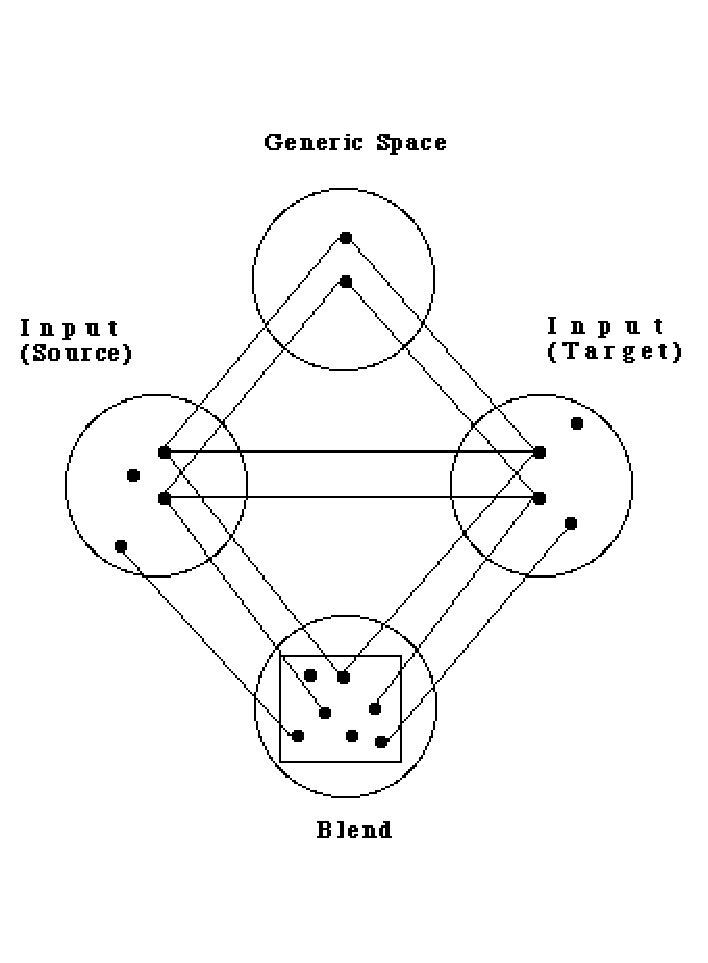
\includegraphics[height=\textheight]{pics/blending.eps}


\myslide{Summary}

\begin{itemize}
\item We routinely understand one thing in terms of another
  \begin{itemize}
  \item Metaphors (LIFE is  JOURNEY)
  \item Image Schema (Everything is spatial)
  \item Mental Spaces (We have multiple contexts)
  \item Cognitive Grammar (Grammar is a metaphor too!)
  \end{itemize}
\end{itemize}


\myslide{Acknowledgments and References}
% \MyLogo{}
 \begin{itemize}
 \item Video from \textit{That Mitchell and Webb Situation} 
\\ Series one episode one
% \item Definitions from WordNet: \url{http://wordnet.princeton.edu/}
  \item Many metaphors on-line at the Conceptual Metaphor Home Page:
\\ \url{http://cogsci.berkeley.edu/lakoff/metaphors/}
%  \item Strict/sloppy identity joke adapted from \textit{Literal-Minded Blog:
% Linguistic commentary from a guy who takes things too literally}.
% \\ \footnotesize\url{http://literalminded.wordpress.com/2011/03/04/you-cant-go-from-strict-to-sloppy/}
 \end{itemize}
 % \item Images from
%   \begin{itemize}
%   \item the Open Clip Art Library: \url{http://openclipart.org/}
%   \item Steven Bird, Ewan Klein, and Edward Loper (2009) 
%      \textit{Natural Language Processing with Python}, O'Reilly Media
%     \\ \url{www.nltk.org/book}
% \end{itemize}
% \item Problems  partially based on exercises from Saeed (2003)
% \end{itemize}

% \myslide{Bibliography}
%  \small
 \bibliographystyle{aclnat}
 \bibliography{abb,mtg,nlp,ling}


\end{document}

%%% Local Variables: 
%%% coding: utf-8
%%% mode: latex
%%% TeX-PDF-mode: t
%%% TeX-engine: xetex
%%% End: 
